\documentclass[aps,prl,twocolumn,reprint,amsmath,amssymb]{revtex4-1}

\usepackage{epsfig,color,graphicx}
\begin{document}
\newcommand{\Ang}{\ensuremath{\mathring{\text{A}}}}
\newcommand{\ltwid}{\mathrel{\raise.3ex\hbox{$<$\kern-.75em\lower1ex\hbox{$\sim$}}}}
\newcommand{\gtwid}{\mathrel{\raise.3ex\hbox{$>$\kern-.75em\lower1ex\hbox{$\sim$}}}}
\newcommand{\ket}[1]{\ensuremath{\vert #1 \rangle}}
\newcommand{\bra}[1]{\ensuremath{\langle #1 \vert}}
\newcommand{\braket}[2]{\ensuremath{\langle #1 \vert #2 \rangle}} % bra-ket inner product
\newcommand{\ketbra}[2]{\ensuremath{\vert #1 \rangle \langle #2 \vert}} % ket-bra outer product
\newcommand{\op}[1]{\ensuremath{\hat{#1}}} % operator
%\newcommand{\sill}{\psi_\mathrm{SILL}}
\newcommand{\sill}{\psi}
\newcommand{\trace}{{\rm Tr}}
\newcommand{\ntilde}{\tilde{n}}
\newcommand{\stilde}{\tilde{s}}
\newcommand{\atilde}{\tilde{\alpha}}
\newcommand{\new}{\color{red}}
\newcommand{\old}{\color{black}}
\newcommand{\bea}{\begin{eqnarray}}
\newcommand{\eea}{\end{eqnarray}}
\newcommand{\br}{\ensuremath{\mathbf{r}}}
\def\nn{\nonumber\\}

\bibliographystyle{apsrev}

\title{Robust [LS] optimization of compact localized orbitals [in DFT]}

\author{Yifei Shi}
\author{Rustam Z. Khaliullin}
\email{rustam.khaliullin@mcgill.ca}
\affiliation{Department of Chemistry, McGill University, 801 Sherbrooke St. West, Montreal, QC H3A 0B8, Canada}

%\date{\today}

\begin{abstract}
Density functional theory based on compact localized nonorthogonal molecular orbitals is a conceptually simple method that can potentially enable low-cost linear-scaling modeling of the electronic structure of molecules and materials with finite energy gap. 
Unfortunately, its development has long been hindered because a compact representation of the electronic ground state is difficult to find in a variational optimization procedure. 
In this work, we showed that the slow and unstable optimization of compact orbitals is due to the nearly-invariant mixing of occupied orbitals that almost entirely but not fully localized within their local vector subspaces. 
%In this work, we identified the origin of the slow and unstable optimization of strictly localized orbitals and developed a simple and robust linear-scaling [optimization] procedure with a low computational overhead. 
We also proposed a simple and practical method for identifying and removing the problematic nearly-invariant modes using an approximate Hessian and, as a result, developed a robust linear-scaling optimization procedure with a low computational overhead.  
We demonstrated the new method is highly efficient yet accurate for a variety of systems ranging from molecular liquids to semi-conductors and insulators.  
%Implications.  %Although this method is not fully variational, it is still accurate enough to produce stable molecular dynamics in systems where chemical reactions happen.
\end{abstract}
\maketitle

\section{Introduction}

Today, Kohn-Sham (KS) density functional theory (DFT) is the most popular electronic structure method. 
The computational cost of the conventional diagonalization-based KS DFT grows cubically with the number of atoms preventing its application to large systems. 
To overcome this limitation, substantial efforts have been directed to the development of linearly-scaling (LS) DFT methods~\cite{goedecker1999linear,bowler2012methods}. 
%RZZK: perhaps it is worth mentioning that construction of the effective KS Hamiltonian is already linear, the current bottleneck is a cubically-scaling procedure for the optimization of electronic degrees of freedom.

In LS DFT methods, the delocalized eigenstates of the effective KS Hamiltonian must be replaced with an alternative set of \emph{local} electronic descriptors. 
Most LS methods explore the natural locality of the one-electron density matrix (DM)~\cite{li1993density, lee1996linear, li2003density, vandevondele2012linear, kussmann2013linear, aarons2016perspective, shao2003curvy}.  
% shao2003curvy: 10.1063/1.1558476
They include the Fermi operator expansion~\cite{goedecker1994efficient,goedecker1995tight}, divide-and-conquer~\cite{yang1991direct,yang1991local}, and direct DM optimization methods~\cite{li1993density, shao2003curvy, vandevondele2012linear}. 
However, the variational optimization of the DM is very inefficient for accurate DFT calculations which require many basis functions per atom~\cite{goedecker1999linear,vandevondele2012linear, arita2014stable, bowler2012methods, khaliullin2013efficient}.
Therefore, the application of DM-based LS methods have been mostly restricted to minimal-basis tight-binding problems~\cite{Richters2014, goringe1997tight, ratcliff2018band}. 
This issue is rectified in optimal-basis DM methods~\cite{skylaris2005introducing, nakata2015optimized, mohr2015accurate} that contract large basis sets into a small number of new localized functions and then optimize the DM in the contracted basis. 
Despite becoming the most popular LS DFT, the efficiency of optimal-basis methods is hampered by the costly optimization of both the contracted orbitals and the DM~\cite{mostofi2003preconditioned}.

From the computational point of view, a direct variation of one-electron orbitals that are strictly localized within predefined spatial regions is preferable because LS can be achieved with significantly fewer variables. %[RZZK: at least for systems with finite band gap]. 
The computational advantages of orbitals-only LS DFT are especially pronounced in accurate calculations that require many basis functions per atom. 
Strictly localized orbitals are also advantageous from the physical point of view because they provide clear, chemically meaningful, transferable description of interactions between atoms or molecules~\cite{RZZK-weitao, stoll1980use, khaliullin2007unravelling, khaliullin2008analysis}. 
%
Such orbitals are known under different names --- localized wave functions~\cite{ordejon1995linear}, nonorthogonal Wannier functions~\cite{weitao,RZZK}, absolutely localized orbitals~\cite{stoll1980use}, orbitals on compact support~\cite{RZZK}, non-orthogonal localized molecular orbital~\cite{weitao}. In this work, they will be referred to as compact localized molecular orbitals (CLMOs) to emphasize that the expansion coefficients of these orbitals in some localized basis set (e.g. numerical atomic orbitals, Gaussian orbitals, psync or RZZK-spline functions) are constrained to be precisely zero outside orbital's predefined localization region.
% RZZK: While we used ALMO -- original name given to these orbitals by Stoll et al. -- to refer to these oribtals we prefer using CLMO in this work to distinguish them from block-diagonal version of ALMO popularized in Head-Gordon et al.  
Unfortunately, the development of promising CLMO-based LS methods has been hindered~\cite{peng2013effective,tsuchida2008ab, fattebert-recent} because of inherently difficult variational optimization of CLMOs~\cite{mauri1993orbital,ordejon1995linear,goedecker1999linear, fattebert2004linear, peng2013effective, tsuchida2008ab, weitao-yang}. 
%There are also other undesirable features, manifesting depending on a particular method: multiple minima, slow convergence with large number of iterations, position of localization centers must be chosen a priori, runaway solutions, charge-conservation issues. These are not exhibited by DM-based methods (Section 3.E of Ref.~\onlinecite{goedecker1999linear}).
%
%Complete CLMO references:
%%%%%% Before Goedecker 1999
% G. Galli and M. Parrinello, Phys. Rev. Lett. 69, 3547 (1992).
% W.-L. Wang and M. Teter, Phys. Rev. B 46, 12798 (1992).
% F. Mauri, G. Galli, and R. Car, Phys. Rev. B 47, 9973 (1993).
% F. Mauri and G. Galli, Phys. Rev. B 50, 4316 (1994).
% P. Ordejon, D. Drabold, M. Grunbach, and R. Martin, Phys. Rev. B 4S, 14646 (1993).
% P. Ordejon, D. Drabold, M. Grunbach, and R. Martin, Phys. Rev. B 51, 1456 (1995).
% W. Kohn, Chem. Phys. Lett. 20S, 167 (1993).
% Further potetially important references -- must be checked:
% E. B. Stechel, A. R. Williams, and P. J. Feibelman, Phys. Rev. B 49, 10088 (1994).
% S. Goedecker and L. Colombo, Phys. Rev. Lett. 78, 122 (1994).
% T. A. Arias, M. C. Payne, and J. D. Joannopoulos, Phys. Rev. Lett. 69, 1077 (1992).
%%%%%% After Goedecker 1999 review:
%%%%%% Jean-Luc Fattebert
% fattebert2000towards https://journals.aps.org/prb/pdf/10.1103/PhysRevB.62.1713
% fattebert2002density https://onlinelibrary.wiley.com/doi/full/10.1002/jcc.10069
% fattebert2004linear https://www.sciencedirect.com/science/article/pii/S0010465504003261
% fattebert2006linear https://journals.aps.org/prb/pdf/10.1103/PhysRevB.73.115124
% oseikuffuor2014accurate https://journals.aps.org/prl/pdf/10.1103/PhysRevLett.112.046401 
%%%%%% Weitao Yang
% Yang, W., 1997, Phys. Rev. B 56, 9294.

In addition to poor convergence, a straightforward optimization of CLMOs, which cannot be constrained to stay both compact and orthogonal~\cite{stoll1980use, RZZK}, often leads to a ``collapsed'' electronic state represented by linearly dependent occupied orbitals~\cite{ordejon1995linear}. 
%
%Furthermore it was also shown in \cite{ordejon1995linear} that the straightforward LMO calculation without using a new energy functional may end up in a set of MOs that are collapsing. And the new energy functionals may lead to multiple minima \cite{kim1995total}. (Perhaps our formulation also has the multiple minima problem)
Figure~\ref{fig:det} shows that such a collapse, indicated by the vanishing determinant of the CLMO overlap matrix, is associated with 
%---caused by or causing---
the convergences problem. 

Several/Numerous efforts were made to resolve these problems. A series of work have focused on using new energy functionals~\cite{mauri1993orbital,kim1995total,ordejon1995linear} that avoid using the inverse of the CLMO overlap matrix. 

%Inclusion of unoccupied orbitals~\cite{kim1995total} or extra optimization variables~\cite{burger2008linear,peng2013effective} has been proposed to mitigate convergence problems. 
In Ref.~\onlinecite{burger2008linear} the authors proposed to apply the absolute energy minimum variational principle~\cite{yang1997absolute} by introducing an extra set of variables. And in a more recent work a preconditioner is used to speed up the convergence~\cite{peng2013effective}.
In an alternative approach, CLMOs can also be described on a real-space mesh~\cite{fattebert2004linear,fattebert2006linear}, and the energy can be evaluated with finite difference. The authors were also able to perform large scale molecular dynamics simulations~\cite{osei2014accurate}.
% kim1995total: They do not resolve the optimization problem, they only create a method that converges to the proper minimum from ANY initial state. They judge convergence by the energy approaching a plato. They need hundreds of steps to produce a well-converged state. They are not converged even then. This can be seen from unstable MD. How do they address the problem of multiple minima? They expand the variational space by including unoccupied orbitals and add the mu-dependent penalty designed to keep the number of electrons constant. They need to optimize mu (chemical potential) as well.
% ordejon1995linear: At each time step of the simulation, the electronic energy was minimized within a tolerance of 10$^{-8}. RZZK: what does it mean? It does not seem that they use the norm of the gradient. Same problem as with kim1995total. Convergence criteria is the energy change, MD is unstable.
%Energy change as the convergence test~\cite{fattebert2000towards, kim1995total, ordejon1995linear}. Not a good convergence criterion. Does not indicate true convergence as shown in Figure~RZZK. Leads to instabilities in AIMD.

We note that in the previously mentioned works, the convergence criteria are always the energy change. However, in this work we use a stronger convergence criteria which is maximum norm of the gradient, which excludes the possibility that the energy enters an unstable plateau during the optimization.

%The origins of the convergence problem have not been described. 
%Dramatically increased computational cost is one reason.

The convergence problem has been reliably solved only for weakly-interacting molecular systems. Tsuchida \emph{et al.} showed~\cite{tsuchida2007augmented,tsuchida2008ab} that CLMOs can be optimized efficiently if they are forced to be orthogonal to  a set of auxiliary tightly localized nonoverlaping orbitals, precomputed and fixed on their molecules. Similar Recently, in Ref.~\onlinecite{khaliullin2013efficient}, a block-diagonal set of orbitals is first optimized and then used to as a projector during optimization of CLMOs in the second step. These two methods have all been successful in improving the convergence by constraining the MOs to be orthogonal to some reference states, thus requiring the reference to be somewhat physically meaningful. RZZK: this only works for weakly-interacting molecular systems (the DOFs projected out already resemble the final occupied states)

Despite multiple potential advantages a reliable orbital-based LS method is still lacking for strongly interacting [nonmetallic] systems. In this work, we propose a new CLMO-based LS DFT method by identifying and projecting out the optimization directions that cause the slow convergence. The new method has the advantage that: 
\begin{itemize}
\item The energy converges fast, and works with systems where interactions are strong.
\item No ``block-diagonal reference" or ``kernel region" are needed like in \cite{tsuchida2007augmented} or \cite{khaliullin2013efficient}.
%(b) The problem of orbital collapse is avoided. (c) Exact inverse of the MO overlap matrix is used, the inversion is linear when the overlap is sparse. This prevents the error introduced by approximate inverse overlap and the problem of multiple minima. 
\item The problem of orbital collapse is avoided. 
\item Although this method is not fully variational and the energy is not the minimum of any energy functional, it still produces stable dynamics for systems involving chemical reactions. 

\end{itemize}

\section{Theory} 

\subsection{Formalism, notation and main assumptions}
 
%In any CLMO method, concepts of electron \emph{localization centers}, often also referred to as fragments, and electron \emph{localization domains} play key roles. 
In the first step, all atoms of a system, its electrons, and atom-centered basis set orbitals --- in our case atomic orbitals (AOs) --- are logically divided into nonoverlapping subsets called \emph{localization centers}, often also referred to as \emph{fragments}. 
For a system with clearly defined molecules, a typical localization center includes all atoms of a single molecule and their associated AOs and electrons. 
For systems that cannot be partitioned into molecules --- the subject of this work --- a localization center can be represented by a single atom. 
As a results of the partitioning, each electron acquires a localization center label. 
Within Kohn-Sham DFT, electrons are described by molecular orbitals (MOs) \ket{\psi_{xi}} whose indices now indicate that orbital $i$ belongs to center $x$. Throughout this work, centers are labeled with Latin letters $x,y,\ldots$ whereas Latin letters $i,j,\ldots$ label MOs. 

In the next step, each atom $A$ is assigned a predefined element-specific radius $R_c(A)$ that defines neighbors of each center in an obvious way: two centers are considered neighbors if there are atoms located within a sum of their radii. 
\emph{Localization domain} for each center is defined as a subset of AOs that are localized on the neighbors of a center \ket{\chi_{\bar{x}\mu}}. In our notation, the bar over a center index $\bar{x}$ refers to all neighbors of this center and basis set orbitals are denoted with Greek letters $\mu,\nu,\ldots$. The basis set orbitals of a localization domain form a subspace in the one-electron vector space and the following projection operator serves as the identity operator on the subspace:
%
\bea
\op{I}_{\bar{x}} = \ket{\chi_{\bar{x}\mu}} S^{\bar{x}\mu,\bar{x}\nu} \bra{ \chi_{\bar{x}\nu}},
\eea
%
where $S^{\bar{x}\mu,\bar{x}\nu}$ is a matrix element of the inverse overlap matrix $S_{\bar{x}\mu,\bar{x}\nu} = \braket{ \chi_{\bar{x}\mu}}{ \chi_{\bar{x}\nu}} $. Note that the conventional tensor notation is used to work with the nonorthogonal orbitals~\cite{head1998tensor}: covariant quantities are denoted with subscripts, contravariant quantities with superscripts, and summation is implied over the same orbital indices but not over the same center and domain indices.
%
By construction a basis set function may belong to several localization domains or, in other words, domains may overlap:
%
\begin{eqnarray}
\label{eq:span}
\hat{I} \neq \sum_{\bar{x}} \hat{I}_{\bar{x}}.
\end{eqnarray}

In the final step, the main approximation of CLMO methods is introduced. It is assumed that the electronic structure of the system can be described accurately by molecular orbitals that are completely localized within domains of their centers
%
\bea
\ket{\psi_{xi}} = \op{I}_{\bar{x}} \ket{\psi_{xi}}
\label{eq:LMO}
\eea
%
Thus this approximation imposes a blocked structure on the matrix of MO coefficients $\mathbf{T}$
%
\bea
\ket{\psi_{xi}} = \ket{\chi_{\bar{x}\mu}} {T^{\bar{x}\mu}}_{xi}
\label{eq:LMOproj}
\eea
%
and offers a way of performing LS calculation directly with MOs. % RZZK: comment how accurate this apprx is expected to be for finite-gap and metallic systems.


\begin{figure}
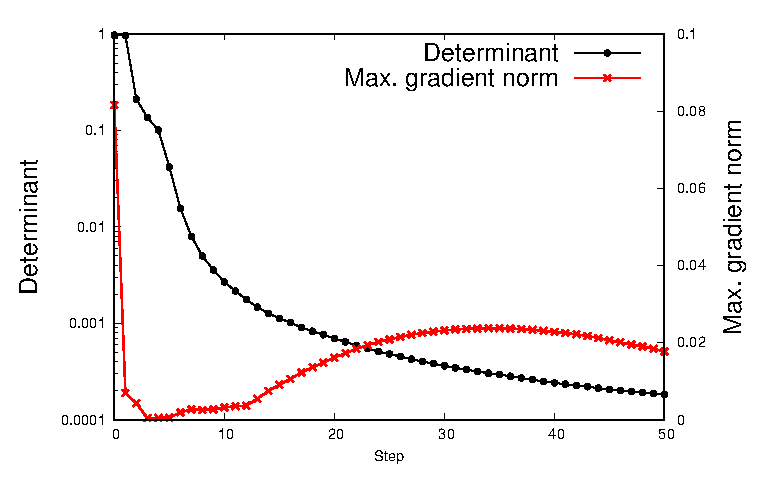
\includegraphics[width=0.5\textwidth]{det}
\caption{
The determinant of the MO overlap matrix, and maximum norm of the energy gradient. In Fig~\ref{fig:det} we show the determinant of the MO overlap matrix and the maximum norm of the energy gradient as a function of the minimization step. PBE/DZVP optimization with the preconditioned conjugate gradient algorithm. Model linear systems of four hydrogen fluoride molecules interacting through hydrogen bonds.}
%RZK: can we also show that the energy plateaus while the gradient is still not converged? 
\label{fig:det}
\end{figure}

In this work, we consider only spin-unpolarized orbitals evaluated at the $\Gamma$-point. The KS DFT energy functional can be written in the conventional way 
% RZZK check the equation
\bea
%E = \trace \left[ \op{R} \left(\op{t} +\op{v} + \op{H} \right) \right] + E_{\text{xc}} - \frac{1}{2}\int v_{\text{xc}}(\br) \rho(\br) d\br
E &=& 2 \trace \left[ \op{R} \op{H} \right] - \frac{1}{2} \int\int \frac{\rho(\br)\rho(\br')}{|\br-\br'|}d\br d\br' \nonumber \\
 &+& E_{\text{XC}} - \int v_{\text{XC}}(\br) \rho(\br) d\br,
\eea
%
where \op{H} is the Kohn-Sham Hamiltonian, \op{R} is the projection operator onto the occupied subspace, and $\rho(\br) = 2\bra{\br}\op{R}\ket{\br}$ is the electron density. \op{R} written to take into account the nonorthogonality of CLMOs
\bea \label{eq:dm}
\op{R} = \sum_{x,y} \ket{\psi_{xi}} \sigma^{xi,yj} \bra{\psi_{yj}},
\eea
%
where $\sigma^{xi,yj}$ is a matrix element of the inverse of the CLMO overlap matrix $\sigma_{zk,wl} = \braket{ \psi_{zk}}{ \psi_{wl}} $. %The one-electron density operator is $\op{D} = 2\op{R}$. 

\subsection{Main problem}

The direct minimization of the energy functional wrt to the variational degrees of freedom --- $\mathbf{T}$ elements --- is a straightforward reliable low-cost method optimization for fully delocalized orbitals ($R_c \rightarrow \infty$)~\cite{galli1992large,OT,GDM, Cayley-minimizer} and completely localized orbitals ($R_c = 0$)~\cite{khaliullin2013efficient}. The preconditioned conjugate gradient algorithm (PCG) is a particularly efficient energy minimizer that requires iterative evaluation of the energy gradient
%
\bea \label{eq:grad}
{G_{\bar{x}\mu}}^{xi} \equiv \frac{\partial E}{\partial {T^{\bar{x}\mu}}_{xi}} = 4 \bra{\chi_{\bar{x}\mu}} (\op{I}-\op{R}) \op{H} \ket{\psi^{xi}}
\eea
%
and only a single inversion of a preconditioner. The latter is typically chosen as an easily-invertible approximation to the exact Hessian. It has been found~\cite{khaliullin2013efficient} that, for the two special cases $R_c \rightarrow \infty$ and $R_c = 0$, the preconditioner defined on domain $\bar{x}$
%
\bea \label{eq:prec}
P_{\bar{x}\mu,\bar{x}\nu} &=& 4 \bra{\chi_{\bar{x}\mu}} (\op{I}-\op{R}) (\op{I} + \op{H})(\op{I}-\op{R}) \ket{\chi_{\bar{x}\nu}} 
\eea
%RZZK - check the prefactor. Is it 2, 4, or 8? Differentiation wrt to T of the same domain
%
provides the same rate of convergence of the PCG algorithm as the exact Hessian but at a fraction of the inversion cost. The relation between the preconditioner in Eq.~(\ref{eq:prec}) and the exact Hessian is presented in the Supplementary Material and Ref.~\onlinecite{stoll1980use}.

\begin{figure*}
\centering
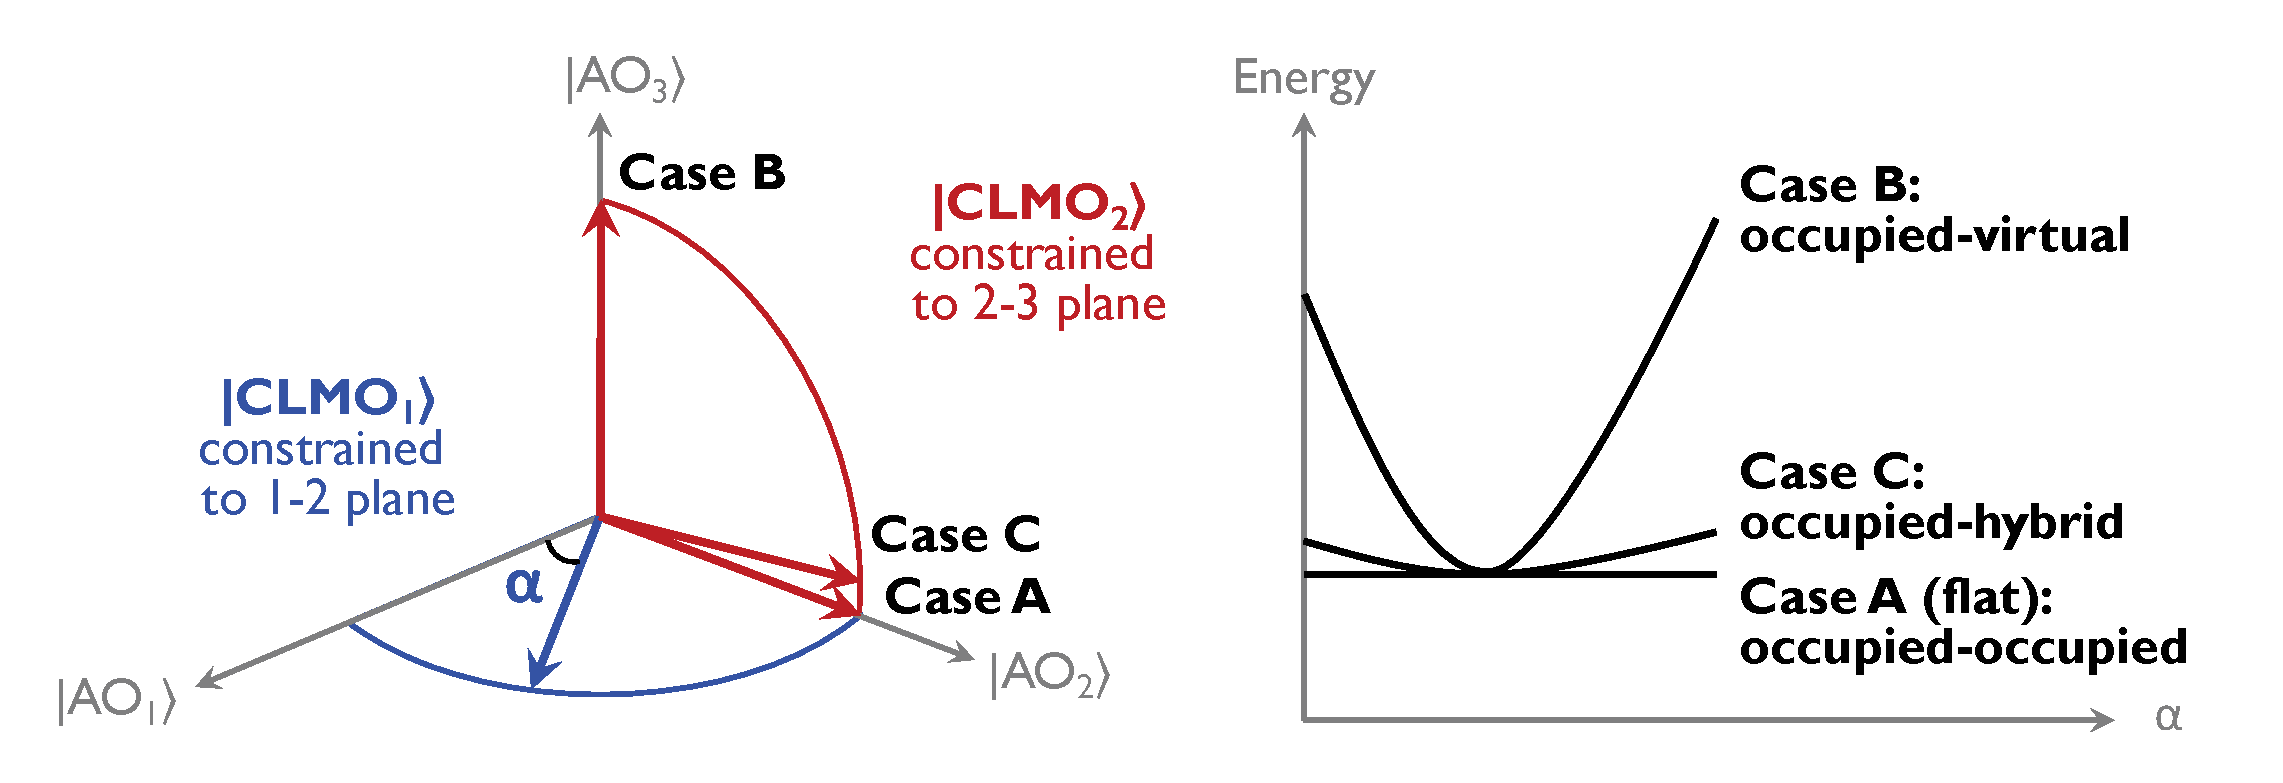
\includegraphics[width=0.8\textwidth]{modes}
\caption{Illustration of the origin of low-curvature modes in a model vector space spanned by three basis set functions \ket{\text{AO}_1}, \ket{\text{AO}_2}, \ket{\text{AO}_3}. The left panel shows \ket{\text{CLMO}_1} (blue) confined to its domain spanned by \ket{\text{AO}_1} and \ket{\text{AO}_2} as well as \ket{\text{CLMO}_2}  (red, three cases) confined to its domain spanned by \ket{\text{AO}_2} and \ket{\text{AO}_3}. The right panel shows the behavior of the energy as a function of the position of \ket{\text{CLMO}_1} --- angle $\alpha$ --- for three typical cases. Case C shows that the low-curvature modes arise when \ket{\text{CLMO}_2}  lies almost entirely in the domain of \ket{\text{CLMO}_1}.}
\label{fig:modes}
\end{figure*}

In the general case of finite $R_c$, the PCG-based optmization of CLMOs has been investigated thoroughly as a low-cost alternative to LS DM-based DFT methods. 
This method was thought~\cite{galli-works,khaliullin2013efficient} to be efficient because both \textbf{T} and \textbf{G} matrices are small (i.e. number of columns is much smaller then the number of rows) and enforced to be extremely sparse. 
In addition to this, the inversion of the approximate Hessian in Eq.~\ref{eq:prec} can be done fast, domain-by-domain. 
%
%RZZK-consider adding a paragraph like this: An important consequence of the CLMO constraints is that both the gradient and the preconditioner are represented by the submatrices confined to their domains. The size of domains is determined only by $R_{c}$ and does not change with the number of molecules. Therefore, the computational cost of the PCG optimization exhibits a linear growth in the limit of large systems. 
%
Unfortunately, the PCG algorithm, as well as all other optimization procedures based on the Newton-Raphson or DIIS-accelerated diagonalizations~\cite{stoll1980use}, suffer from the aforementioned slow convergence and orbital collapse problems. 
%
A closer inspection of the eigenvalues of the preconditioner obtained by solving the generalized eigenproblem for each domain 
%
\bea
%\mathbf{P}_{\bar{x}} \mathbf{A}_{\bar{x}} =  \mathbf{S}_{\bar{x}} \mathbf{A}_{\bar{x}} \Lambda_{\bar{x}} \\
P_{\bar{x}\mu,\bar{x}\nu} {A^{\bar{x}\nu}}_{xp} =  S_{\bar{x}\mu,\bar{x}\kappa} {A^{\bar{x}\kappa}}_{xp} \Lambda_{xp},
\label{eq:gev}
\eea
%
reveals the origin of this and other closely related previously reported problems~\cite{goedecker1999linear}. 
The eigenvalues, which approximate the energy curvature along the optimization direction \ket{d_{xp}} given by the corresponding eigenvector, ${A^{\bar{x}\nu}}_{xp} \equiv \braket{\chi^{\bar{x}\nu}}{d_{xp}}$, can be divided into three categories according to their magnitudes. 
Zero eigenvalues in the first category represent optimization directions towards occupied orbitals localized completely within the same domain (Figure~\ref{fig:modes}, case A). 
As expected the energy is invariant along these occupied-occupied mixing modes. 
The second category includes large nonzero eigenvalues that represent the optimization in the direction toward unoccupied orbitals (Figure~\ref{fig:modes}, case B) of the domain. 
These two categories are the only present in the rapidly converging optimization of fully delocalized orbitals ($R_c \rightarrow \infty$) and completely localized orbitals ($R_c = 0$). 
The eigenvalues classified as the third category are extremely small but nonzero (Fig~\ref{sfig:hesseig} in the Supplementary Material). 
They appear only for finite $R_c$ when orbitals on different domains share basis set functions. 
The optimization along these low-curvature nearly-invariant directions is difficult to converge because various analytical approximations (e.g. approximate Hessian, quadratic linear search) and numerical noise (e.g. finite DFT grids) make calculations  imprecise. 
In other words, optimization with finite $R_c$ becomes ill-conditioned and the low-curvature modes represents the major barrier to the practical use of promising orbital-based LS DFT methods. 


\subsection{Nature of low-curvature modes} \label{marker:nature} 

What is the physical origin of the low-curvature optimization modes? 
It has been suggested previously~\cite{goedecker1999linear} that the sluggish optimization in orbital-based LS DFT is due to the inexact invariance of the energy wrt the mixing of occupied orbitals. 
Although this might indeed present a problem for a series of functionals based on DMs that are not fully idempotent~\cite{Galli-90s,grumbach} the DM used in this work is constructed with the inverse of the overlap matrix and, therefore, is properly idempotent and exactly invariant to the mixing among occupied states. 

We instead suggest that the low-curvature optimization modes represent mixing in \emph{hybrid} directions, which are neither occupied nor virtual. From the point of view of the vector space of a single domain $\bar{x}$, these directions exist because CLMOs of neighbor centers are only partially localized on $\bar{x}$. 
Hybrid directions associated with CLMOs that are almost but not entirely localized on a domain are expected to be particularly problematic and illustrated in Figure~\ref{fig:modes}, case C. 

Our hypothesis can be verified by calculating the residue $\Delta$ of the small-curvature directions \ket{d_{\bar{x}p}} in the unoccupied space projected onto subspace of a domain:
%
\bea
\label{eq:residue}
\Delta_{\bar{x}p} \equiv \bra{d_{\bar{x}p}} \op{I}_{\bar{x}} - \op{R}_{\bar{x}} \ket{d_{\bar{x}p}}, 
\eea
%
where $\op{R}_{\bar{x}}$ is a projector constructed from the occupied CLMOs of the neighbors truncated to the subspace $\bar{x}$ with operator $\op{T}_{\bar{x}} \approx \op{I}_{\bar{x}}$
\bea
{R}_{\bar{x}} &=& \sum_{y,z \in \bar{x}} \op{T}_{\bar{x}} \ket{\psi_{yi}} \sigma_{\bar{x}}^{yi,zj} \bra{\psi_{zj}} \op{T}_{\bar{x}}
%R^{\bar{x}\mu,\bar{x}\nu} &\equiv& \bra{\chi^{\bar{x}\mu}} \op{R}_{\bar{x}} \ket{\chi^{\bar{x}\nu}} \\
\label{eq:C}
\eea
%
and $\sigma_{\bar{x}}$ is the overlap matrix of the truncated orbitals.
%%
%\bea
%\left(\sigma_{\bar{x}}\right)_{yi,zj} = \bra{\psi_{yi}} \op{I}_{\bar{x}} \ket{\psi_{zj}}
%\eea
%%

Our hypothesis implies that $\Delta$ should be small for all small-curvature eigenvectors. 
Figure~\ref{fig:projection} shows that indeed the small-curvature modes indeed have lie outside the unoccupied space for a variety of materials (see Supplementary Material for more details). 
It is also interesting to note that the unoccupied fraction of the low-curvature modes increases with increasing strength of inter-center delocalization, that is, with the degree of covalency of interatomic bonding. %RZZK: detailed expalnation why this is so.
Thus the optimization along the low-curvature modes represents mixing of an occupied CLMO with occupied orbitals that are not fully localized on its domain. 
Unsurprisingly, such orbital variations often lead to linear dependencies among occupied orbitals and eventual collapse of the optimization. 

\begin{figure}
\centering
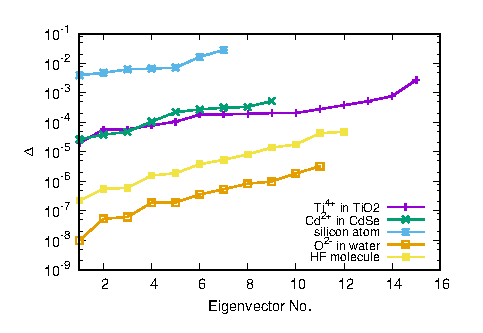
\includegraphics[width=0.5\textwidth]{residue}
\caption{
The norm of the projection of the small-curvature modes on the unoccupied subspace of a domain. 
Preconditioner eigenvectors with the eigenvalues smaller than 0.02~a.u. are chosen as small-curvature modes. 
The following localization ceneters are considered: Ti$^{4+}$ ions in the TiO$_2$ rutile lattice, Cd$^{2+}$ ions in the CdSe Wurtzite lattice, Si atom in the diamond silicon lattice, O$^{2-}$ in a water tetramer system, hydrogen fluoride molecule in a linear tetramer system. 
The BLYP/TZV2P level of theory is used for water and PBE/DZVP in all other tests.}
%RZK: The legend should mirror the caption: "Ti$^{4+}$ in TiO$_2$" and so on. 
\label{fig:projection}
\end{figure}

The proposed explanation of the nature of the low-curvature modes is consistent with the fact that, for molecular partitioning, their number is equal to the sum of occupied orbitals on the neighbor centers. It also explains why the two-stage procedure of Ref.~\onlinecite{khaliullin2013efficient} works so well for molecular systems. In the first stage of this procedure, $R_c$ is set to zero and the resulting block-diagonal orbitals \ket{\psi_{xi}^{0}} are optimized variationally to construct the occupied space projector $\op{R}^{0}$. This projector is then fixed, $R_c$ is reset to its original finite value to allow intercenter electron delocalization, and the following trial CLMOs are optimized with respect to the elements of $\mathbf{\bar{T}}$ matrix:
%
\bea
\ket{\psi_{xi}} &=& \ket{\psi_{xi}^{0}} + \op{I}_{\bar{x}} (\op{I} - \op{R}^{0} ) \ket{\chi_{\bar{x}\mu}} \bar{T}^{{\bar{x}\mu}}_{xi}
\label{eq:LMOproj}
\eea
%
For the CLMOs of this form, the gradient and preconditioner  
%
\bea \label{eq:grad-bar}
\bar{G}{_{\bar{x}\mu}}^{xi} &\equiv & \frac{\partial E}{\partial \bar{T}^{{\bar{x}\mu}}_{xi}} = 
%4 \bra{\chi_{\bar{x}\mu}} \op{Q}_{\bar{x}}^{0} (\op{I}-\op{R}) \op{H} \ket{\psi^{xi}} = \nonumber \\
%&=& 
\bra{\chi_{\bar{x}\mu}} \op{Q}_{\bar{x}}^{0} \ket{\chi^{\bar{x}\nu}} {G_{\bar{x}\nu}}^{xi}
\eea
%
\bea \label{eq:prec-bar}
\bar{P}_{\bar{x}\mu,\bar{x}\nu} &=& 
%\bra{\chi_{\bar{x}\mu}} (\op{I} - \op{R}^{0} ) \ket{\chi^{\bar{x}\lambda}}  P_{\bar{x}\lambda,\bar{x}\alpha} \bra{\chi^{\bar{x}\alpha}} (\op{I} - \op{R}^{0} ) \ket{\chi_{\bar{x}\nu}}
\bra{\chi_{\bar{x}\mu}} \op{Q}_{\bar{x}}^{0} \ket{\chi^{\bar{x}\lambda}}  P_{\bar{x}\lambda,\bar{x}\alpha} \bra{\chi^{\bar{x}\alpha}} \op{Q}_{\bar{x}}^{0} \ket{\chi_{\bar{x}\nu}}
\eea
%RZZK: define \op{P} and check the constant here again.
are related to those in Eqs.~(\ref{eq:grad}) and~(\ref{eq:prec}) for the straightforward CLMO expansion (\ref{eq:LMOproj}) via domain-specific projectors
%
\bea \label{eq:q0}
\op{Q}_{\bar{x}}^{0} &\equiv & \op{I}_{\bar{x}} (\op{I} - \op{R}^{0} ) \op{I}_{\bar{x}}
\eea
%
For molecular systems, $\op{Q}_{\bar{x}}^{0}$ is key to convergence. The present work suggests that this is because $\op{Q}_{\bar{x}}^{0}$ satisfies two important requirements. First, it is constructed from CLMOs fully localized on their centers and thus ensures that each domain contains an integer number of occupied dimensions. Second, it is constructed from $\op{R}^0$ that is already close to the final converged DM and, therefore, removes the optimization modes that coincide with low-curvature directions.  

Unfortunately, the two-stage approach does not work for systems with strong covalent bonds between localization centers (i.e. atoms). This is illustrated in Figure~\ref{fig:convergence} for the cadmium selenide lattice. The main reason for the deteriorating convergence is the inability of $\op{R}^0$, which is constructed from the block-diagonal CLMOs, to represents the low-curvature modes in the later stages of the optimization adequately. 

\subsection{Proposed solution to the optimization problem}

%[In fact, it is difficult to construct a trial CLMO that is both simple and .] 

Instead of performing the two-stage procedure we propose to solve the problem of sluggish convergence by detecting the low-curvature modes directly by diagonalizing the approximate Hessian in Eq.~(\ref{eq:prec}) and avoiding the optimization along these modes altogether. Although this procedure does not produce fully optimized orbitals they are still expected to provide accurate representation of the ground state. This is because the low-curvature modes are associated mostly with mixing of occupied and nearly-occupied orbitals and, therefore, are expected to be \emph{shallow} optimization directions. That is, they are unlikely to produce a noticeable variational decrease in the energy.

To filter out low-curvature modes we construct a projector
%
\bea
%L^{\bar{x}\mu,\bar{x}\nu} &=& {A^{\bar{x}\mu}}_{xp} \Theta_{xp} {A^{\bar{x}\nu}}_{xp} \\
\op{Q}_{\bar{x}} &=& \ket{d_{\bar{x}p}} \, \Theta\left[ \Lambda_{\bar{x}p} - \Lambda_c \right] \bra{d_{\bar{x}p}},
\eea
%
where $\Theta$ is the unit step function 
\bea
\Theta \left[\Lambda_{\bar{x}p} - \Lambda_c \right] =
\begin{cases} 
      0 & \Lambda_{\bar{x}p} \leq \Lambda_c ,\\
      1 & \Lambda_{\bar{x}p} \geq \Lambda_c
\end{cases}
\eea
%
and $\Lambda_c$ is the curvature threshold below which the optimization mode is classified as a low-curvature mode. This projector is then applied to the gradient and preconditioner in the PCG optimization algorithm
%
\bea
\tilde{G}{_{\bar{x}\mu}}^{xi} &=& \bra{\chi_{\bar{x}\mu}} \op{Q}_{\bar{x}} \ket{\chi^{\bar{x}\nu}} {G_{\bar{x}\nu}}^{xi} \label{eq:grad-lcp} \\
%
\tilde{P}_{\bar{x}\mu,\bar{x}\nu} &=& \bra{\chi_{\bar{x}\mu}} \op{Q}_{\bar{x}} \ket{\chi^{\bar{x}\lambda}}  P_{\bar{x}\lambda,\bar{x}\alpha} \bra{\chi^{\bar{x}\alpha}} \op{Q}_{\bar{x}} \ket{\chi_{\bar{x}\nu}} \label{eq:prec-lcp}.
\eea
%
As a result, the PCG optimization procedure neglects low-curvature modes. 
%Hopefully, the energy changes associated with them are  small. 

\begin{figure}
\centering
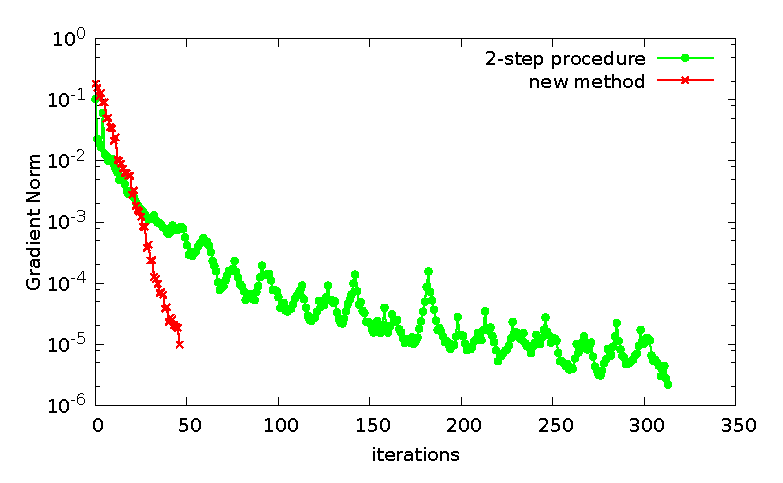
\includegraphics[width=0.5\textwidth]{convergence}
\caption{The maximun norm of the energy gradient for the PBE/DZVP basis~\cite{vandevondele2007gaussian} optimization of the CLMOs for the hexagonal wurtzite CdSe lattice. $R_c = 3.5$~{\AA}. Modes with the preconditioner eigenvalues lower than 0.05~a.u. are removed from the optimization.} 
%The difference in the ground state energy for the two methods is 0.03 kJ/mol per Cd atom.
%RZZK: Explain the legend in the caption. 
\label{fig:convergence}
\end{figure}

We will refer to the new method based on Eqs.~(\ref{eq:grad-lcp}) and (\ref{eq:prec-lcp}) as low-curvature projector (LCP) method.
%RZZK- this would be a good place to say a couple of words about the connection of LCP to the two-stage procedure, its trial CLMOs and its weaknesses: dependence on optimization path, absence of a well-defined trial wavefunction.
%Use this?: We note that upon applying the LCP $\op{Q}_{\bar{x}}$ on the gradient, the final energy is no longer fully variational: the gradient is only zero in diretions that significantly change the energy. It also implies that the energy will depend on the optimization path.

%RZZK: This projection can be understood as a relaxed orthogonality constrain for the CLMOs. 

%RZZK: Add to discussion: One weakness of defining CLMO domains \emph{a priori} in this way is that at least rough idea about the electron distribution in a system is required to assign electrons to localization centers and domains. Such a procedure is, of course, not applicable to systems in which the exact bonding properties are unknown.

%RZZK: Discuss advantages and weaknesses of the new method: (a) We are giving up a strict energy functional. As a consequence, the final energy may depend on the optimization path (i.e. how often the PCG is restarted and preconditioner is recalculated). However, we demonstrate that the dependence of the energy on optimization path is insignificant and the final energy is close to the ground state. Moreover, the proposed method passes even more stringent test: it appears to produce stable molecular dynamics trajectories. As stated before, the filtered directions should be primarily occupied-occupied mixing, so that physically meaning full directions are not neglected and the final state is close to the true ground state. 

%RZZK: The physical meaning of Eq~\ref{eq:approxq} is a modified orthogonality constrain for LMOs. Orthognality and locality has generally been considered as competing properties: strict orthogonality leads to decaying tails, and for LMOs no orthogonality constrains are imposed except for MOs within a fragment. However, this causes the convergence problem previously mentioned: LMOs without orthogonality tends to collapse. Although global orthogonality cannot be achieved, we suggest a local orthogonality constrain, that the projection of MOs onto each fragment $x$ should be orthogonal. Unlike the case for none-local MOs, not every physical state can be transformed into such state.

%RZZK: While many previous works~\cite{RZZK} dealt with weakly-interacting fragments (e.g. molecules) the approach here represents the ultimate atomic partitioning scheme.

\subsection{Implementation}

The procedure for finding and projecting out the low-curvature modes is implemented in the CP2K software package~\cite{cp2kgeneral}. CP2K relies on the mixed Gaussian and plane wave representation of the electronic degrees of freedom~\cite{vandevondele2005quickstep} and is an ideal platform for the new orbital-based LS method: just a few tightly-localized Gaussian AOs can provide an accurate representation of CLMOs, whereas plane waves ensure a fast LS construction of the KS Hamiltonian for large systems.

All matrix multiplications are performed with the DBCSR library~\cite{borvstnik2014sparse} designed for parallel linear-scaling handling of sparse matrices. 
A special care is taken to reduce the computational overhead of the optimization procedure for large Gaussian basis sets. 
To this end, the order of matrix multiplications in Eqs.~(\ref{eq:grad-lcp}) and (\ref{eq:prec-lcp}) is chosen to avoid steps that scale cubically with the size of the Gaussian basis set. 
The diagonalization of the preconditioner matrices is done independently for each domain. 

It is important to note that the construction of the DM requires the inversion of the CLMO overlap matrix. 
This matrix is small and its size is independent of the size of the basis set. 
However, it is not confined to individual domains. This inversion is carried out using the iterative Hotelling method~\cite{hotelling1943some} that is based entirely on matrix multiplications and becomes LS when the system is large and the CLMO overlap and its inverse are sparse. 

Because of the similarity between the new method and the ALMO SCF for molecular systems only minor modifications in the existing ALMO DFT module of CP2K are necessary. The main difference between the algorithms in the two approaches is that the PCG optimization of CLMOs in the LCP method might need more frequent re-evaluation and inversion of the preconditioner.

%RZZK: PCG is restarted once in a while or it can be restarted quite often. If it is restarted and precond is evaluated on every step it become a Newton-Raphson with approximate Hessian.

\subsection{Computational details}

RZK: detailed description of computational procedures? E-cutoff, molopt. important numerical settings?

\section{Results and discussion}

%\subsection{Convergence}

Figure~\ref{fig:convergence} shows that the new optimization procedure converges rapidly for the hexagonal CdSe lattice -- a particularly challenging case for LS methods considering the small band gap of this material and strong interactions between atoms. 
In contrast, it is difficult to achieve convergence for the two-stage method described in Ref.~\cite{khaliullin2013efficient}. 
It is also important to note that the final energy obtained with the new method is close to that obtained using the two-stage method. %RZK-This is not a fair comparison because the two-stage struggles to optimize the neglected DOFs. Add comparison to the fully delocalized reference?

%\subsection{Accuracy} 

The accuracy of the LCP energies as a function of $R_c$ is shown in Figure~\ref{fig:accuracy} for several challenging systems with strong interaction and significant electron delocalization between fragments: CdSe in the hexagonal wurtzite lattice; liquid water in which each atom is treated as a fragment; silicon in the cubic diamond lattice. 
Figure~\ref{fig:accuracy} demonstrates that the energy converges to the correct ground state energy as $R_c$ increases and that the error of the localization constraints imposed on electrons is small. The insets in Figure~\ref{fig:accuracy} also shows that the error of projecting out the low-curvature optimization modes is even small than that introduced by finite $R_c$. This confirms our hypothesis that the low-curvature directions do not produce a noticeable decrease in the energy.

\begin{figure}
\centering
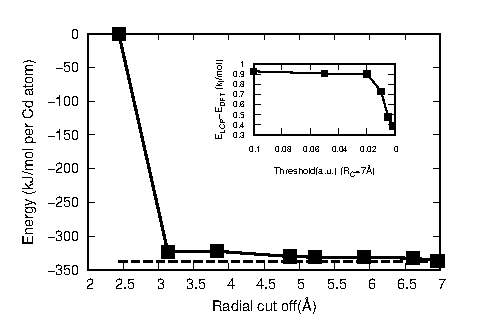
\includegraphics[width=0.35\textwidth]{CdSe_conv}
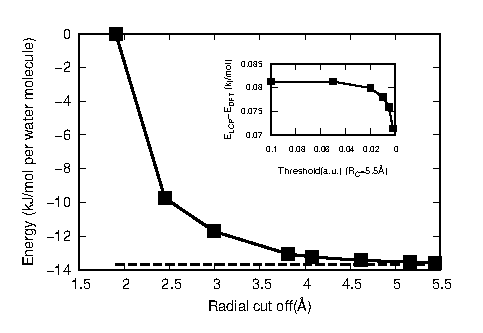
\includegraphics[width=0.35\textwidth]{H2O_conv}
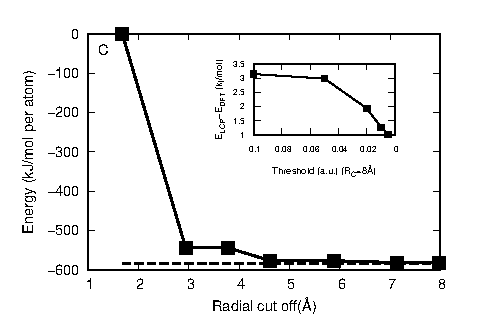
\includegraphics[width=0.35\textwidth]{Si_conv}
%RZK: Letters A., B., C. in the figure must be in the top left corner. See journal formatting.
\caption{Energy from the low-curavture projector and the dependence on the localization radii $R_c$ for: A. PBE/DZVP calculation for the hexagonal wurtzite phase of CdSe, B. BLYP/TZV2P calculation for atomically-partitioned liquid water, C. PBE/DZVP calculation for the cubic diamond phase of silicon. The convergence criteria is $\vert\vert \tilde{G} \vert\vert_{\text{max}} < 10^{-5}$~a.u. The zero energy is set at the energy of the fully optimized block-diagonal CLMOs (R$_c = 0$). Dashed line shows the reference energy of conventional DFT calculation (E$_{\text{DFT}}$) without localizatioin constrains (R$_c\rightarrow \infty$). 
Inset: LCP energy dependence on the low-curvature threshold $\Lambda_c$ at a fixed $R_c$. The zero energy is set at E$_{\text{DFT}}$.}
\label{fig:accuracy}
\end{figure}

To demonstrate the accuracy of the LCP energies further, we performed a 500~K Monte Carlo (MC) simulation of silicon in the cubic diamond lattice with a defect created by replacing two neighboring silicon atoms with two carbon atoms. Figure~\ref{fig:mc} shows that the silicon-silicon radial distribution function (RDF) at equilibrium almost perfectly reproduces that calculated using conventional DFT methods for fully delocalized electrons. 

\begin{figure}
\centering
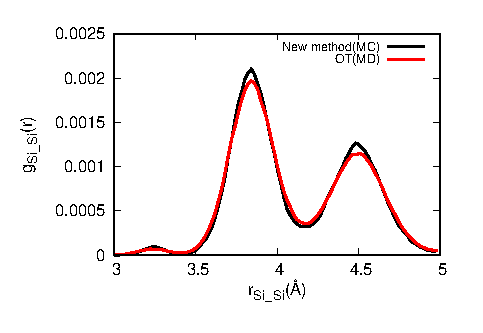
\includegraphics[width=0.45\textwidth]{rdf_si}
\caption{Silicon-silicon RDF calculated for the cubic diamond phase of silicon with carbon atoms introduced to create a point defect. XC/basis simulations are performed at $T=500$~K with the conventional orbital-transformation~\cite{RZK-OT} method for the delocalized electrons and the LCP method with $R_c = 6$~\AA\ and $\Lambda_c = 0.02$~a.u. The system includes 62 silicon atoms and two carbon atoms.}
\label{fig:mc}
\end{figure}

%\subsection{Stable molecular dynamics simulations} 

Molecular dynamics (MD) simulations present an even more stringent test on the accuracy of the LCP method. While minor errors in energies are not crucial in fixed-nuclei calculations, geometry optimizations, and Monte-Carlo simulations they tend to accumulate in MD trajectories leading to non-physical sampling and eventual failure. Accurate calculation of forces is therefore crucial for molecular dynamics simulations, the stability of which are judged by the accumulated drift in various conserved quantities. Although CLMOs obtained with the LCP method are not strictly variational we chose to neglect this error and invoke the Hellmann--Feynman theorem~\cite{feynman1939forces} in the calculation of atomic forces. An LCP-based MD test was performed for a protonated water nanocluster containing 62 water molecules and two protons. In the course of a three-picosecond MD simulation, the 2 protons hop around breaking and forming covalent bonds with water molecules. To reproduce motion of protons around the nanodroplet each atom was treated as a localization center. Setting $R_c = 4$~\AA\ and $\Lambda_c = 0.005$~a.u. produces sufficiently optimized CLMOs to ensure the stability of the MD simulation. Figure~\ref{fig:md} shows that the drift in the conserved quantity is acceptably small compared to the magnitude of the fluctuations in the potential energy. The applicability of the LCP method in MD simulations will be explored further especially in conjunction with the modified Langevin integrator method~\cite{scheiber2018communication}. 

%RZZK: This partitioning allows to study chemical processes in the course of simulations without resorting to complex and unreliable schemes that redefine molecular fragments on-the-fly.

\begin{figure}
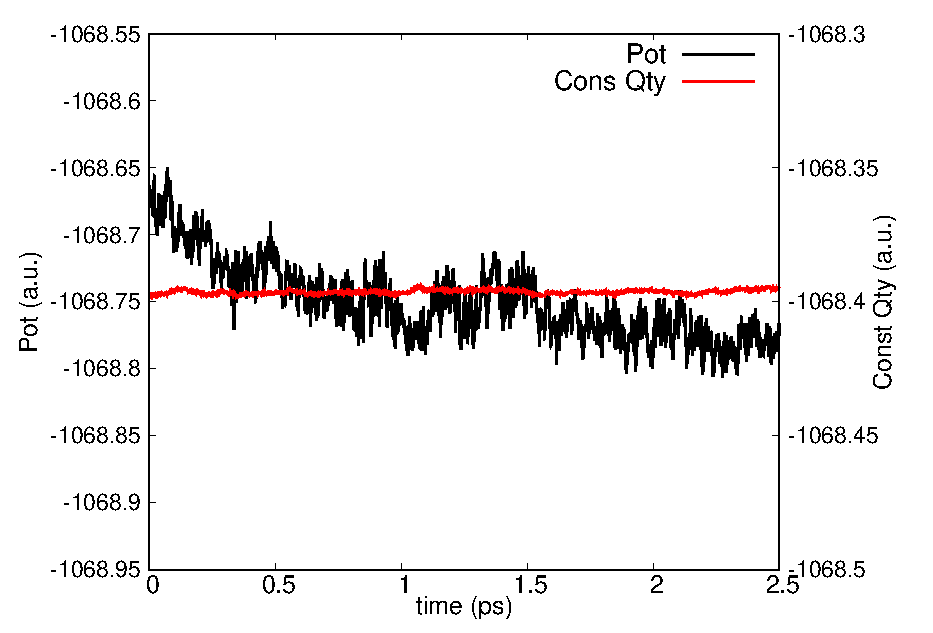
\includegraphics[width=0.45\textwidth]{const.eps}
\caption{The potential energy and the conserved quantity in a LCP-based MD simulation of a protonated water nanocluster $\text{(H}^{+}\text{)}_2\text{(H}_2\text{O)}_{62}$. The temperature of the NVT simulations is set to 298~K and controlled by a canonical velocity re-scaling thermostat~\cite{bussi2007canonical} with the coupling time constant of 50~fs. The potential energy and conserved quantity are shifted for clarity.}
\label{fig:md}
\end{figure}


%\subsection{Computational efficiency}

To test the computational efficiency of the newly designed method, we compared its performance to the orbital transformation (OT) method~\cite{weber2008direct,vandevondele2003efficient} --- a well-optimized low-prefactor cubic scaling DFT method for conventional fully delocalized orbitals. The calculation is done for the hexagonal CdSe system of different sizes. $R_c$ is set to 3.5~{\AA}, which is large enough to accurately describe the electronic structure of the system (Figure~\ref{fig:accuracy}) and $\Lambda_c = 0.02$~a.u. Figure~\ref{fig:scaling} demonstrates that the LCP method is asymptotically LS. The LS regime is achieved when the MO overlap matrix and its inverse are sparse. For a dense 3D system like CdSe it takes on the order of $\sim$3000 atoms. 
%RZK: compare timing to that of a typical DM method. What EPS_DEFAULT and EPS_FILTER did you use to perform timing benchmark? 
%Yiei: EPS_DEFAULT: 1E^-12 EPS_FILTER: 1E-8

\begin{figure}
\centering
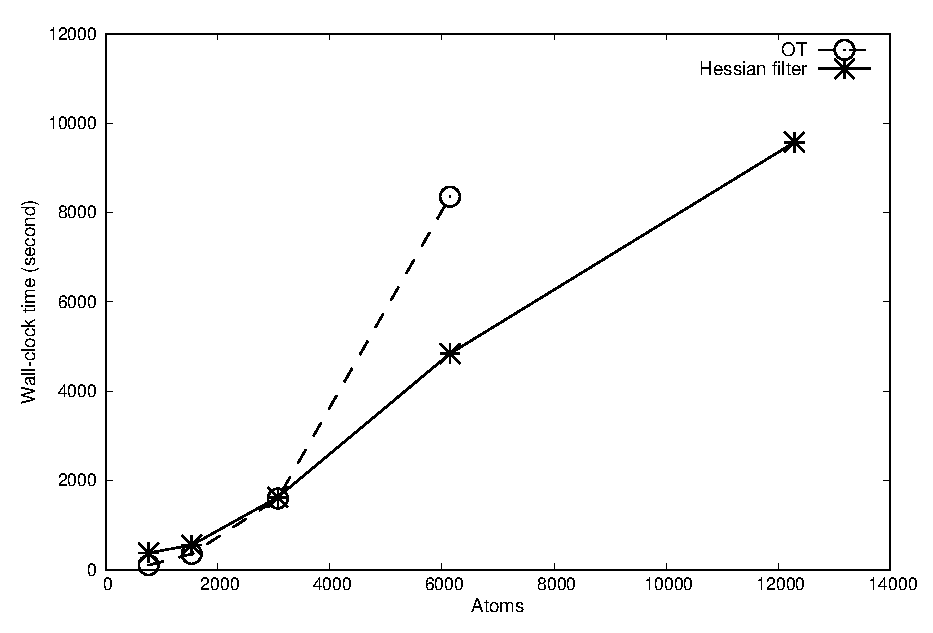
\includegraphics[width=0.45\textwidth]{timing}
\caption{CLMO optimization timing benchmark for the hexagonal CdSe lattice. The PBE/DZVP calculation with $R_c=3.5$~{\AA} and $\Lambda_c = 0.02$~a.u. is done on 256 compute cores.}
\label{fig:scaling}
\end{figure}


\section{Conclusions} 

This work presents a new linear-scaling DFT method based entirely on the straightforward variational optimization of localized molecular orbitals. 
Unlike many existing LS methods, the method does not perform the typical concomitant variation of the density matrix and thus has a substantially lower computational cost. 
The notorious convergence problem that has plagued orbital-based LS DFT methods is resolved by avoiding the optimization of orbitals along low-curvature modes -- the directions associated with tiny eigenvalues of the electronic Hessian. 
An efficient procedure is designed to identify the low-curvature modes on-the-fly without the computationally costly construction and diagonalization of the Hessian. 
It is also shown that the low-curvature modes --- an unavoidable repercussion of imposing localization constraints --- can be safely neglected because they are associated with the mixing of nearly occupied states and do not produce a noticeable variational decrease in the energy. 

The new methodology, which is expected to be applicable to systems with nonvanishing band gap, is tested on a variety of materials including rutile phase of titania, cubic diamond phase of silicon with defects, and hexagonal phase of cadmium selenide. 
These tests demonstrate that the method is accurate and efficient even when localization centers are represented by single atoms and there are strong covalent interaction between the centers. 
Furthermore, preliminary tests on protonated water nanoclusters suggest that the atomic partitioning does not present problems for the new method and it is sufficiently robust to enable stable molecular dynamics simulation of bond-breaking and formation processes. 

The developed LS DFT method is expected to have a significant impact on computational modeling of complex systems due to its low computational overhead, enabling calculations on previously inaccessible time and length scales and making completely new chemical phenomena amenable to simulations.

\section{Acknowledgments} The research was funded by the Natural Sciences and Engineering Research Council of Canada through the Discovery Grant (RGPIN-2016-05059). The authors are grateful to Compute Canada for computer time.

\bibliography{negref}

\section{Supplemental Material}

\setcounter{equation}{0}
\setcounter{figure}{0}

\renewcommand{\theequation}{S\arabic{equation}}
\renewcommand{\thefigure}{S\arabic{figure}}

\subsection{Details of matrix equations}
Matrix equations clarify more compact operator expression used in the main text. 

%The energy:
%\bea
%E[\{\psi_i\}] &=& 2\sum_{i,j} (\sigma^{-1})_{ij}\int \psi_i (\br) h(\br) \psi_j(\br) d\br \nonumber \\
%&+& \frac{1}{2} \int \int \frac{\rho(\br)\rho(\br')}{|\br-\br'|}d\br d\br' + E_{XC}[\rho] 
%%\\
%%&+& 2\sum_{i,j} (\sigma^{-1})_{i,j}\int \psi_i(\br) \psi_j(\br) d\br \nonumber
%\eea
%%
%where $h(\br)$ is the combine kinetic and nuclear-electron attraction energy operator
%%
%\bea
%h(\br) \equiv -\frac{1}{2}\nabla^2 + v_{\text{ext}}({\br}),
%\eea
%%
%$\rho(\br)$ is the electron density
%%
%\bea
%\rho(\br) \equiv 2 \sum_{i,j} (\sigma^{-1})_{ij} \psi_i(\br) \psi_j(\br) ,
%\eea
%%
%and $\sigma$ is the CO overlap matrix
%%
%\bea
%\sigma_ij \equiv  \int \psi_i (\br) \psi_j(\br) d\br .
%\eea
%%

Contravariant density matrix:
%
\bea
\mathbf{R} = \mathbf{T} \sigma^{-1} \mathbf{T}^{\dagger}
\sigma = \mathbf{T}^{\dagger} \mathbf{S} \mathbf{T}
\eea
%
or, using the element by element notation,
%
\bea
R^{w\mu,z\nu} = \sum_{x,y}{T^{\overline{wx}\mu}}_{xi} \sigma^{xi,yj} {T^{\overline{zy}\nu}}_{yj}
\eea

The gradient for domain $\bar{x}$
%
\bea
\mathbf{G}_{\bar{x}x} = 4 \left[(\mathbf{I}-\mathbf{SR}) \mathbf{H} \mathbf{T}\sigma^{-1} \right]_{\bar{x}x}
\eea
%
or
%
\bea
{G_{\bar{x}\mu}}^{xi} = 4 \left[(\mathbf{I}-\mathbf{SR}) \mathbf{H} \mathbf{T}\sigma^{-1}\right]{_{\bar{x}\mu}}^{xi}
\eea
%

The preconditioner for domain $\bar{x}$ 

%
\small {
\bea
P_{\bar{x}\bar{x}} &=& s_x \left[(\mathbf{I}-\mathbf{SR}) \mathbf{H}(\mathbf{I}-\mathbf{RS}) + (\mathbf{I}-\mathbf{SRS})\right]_{\bar{x}\bar{x}} 
\eea 
%
\bea
P_{\bar{x}\mu,\bar{x}\nu} &=& s_x \left[(\mathbf{I}-\mathbf{SR}) \mathbf{H}(\mathbf{I}-\mathbf{RS}) + (\mathbf{I}-\mathbf{SRS})\right]_{\bar{x}\mu,\bar{x}\nu} 
\eea 

$\bar{x}$-coefficients of the $y$-centered orbitals projected onto $\bar{x}$-space are determined by
%
\bea
\op{I}_{\bar{x}} \ket{\psi_{yi}}  &=& \ket{\chi_{\bar{x}\mu}} S^{\bar{x}\mu,\bar{x}\nu} \braket{ \chi_{\bar{x}\nu}}{ \chi_{\bar{y}\lambda}}\, {T^{\bar{y}\lambda}}_{yi} = \nonumber \\
 &=& \ket{\chi_{\bar{x}\mu}} \left[ S^{\bar{x}\mu,\bar{x}\nu} S_{\bar{x}\nu,\bar{y}\lambda} {T^{\bar{y}\lambda}}_{yi} \right]
\eea 
}
%
Note that coefficients outside $\bar{x}$ may be nonzero but we do not need them.

\subsection{Generalized eigenvalues of Hessian, and physical meaning of low-curvature-projector}

Here we further illustrate the origin of slow converging modes by looking at the (generalized) eigenvalues of the Hessian in the calculation of a realistic system. Fig~\ref{sfig:hesseig} shows the cases of (a)completely delocalied calculation, where the eigenvalues are either 0(corresponding to a occupied-occupied mixing) or significanly large(occupied-virtual mixing). (b) Straight forward CLMO calculation, where the eigenvalue spectrum is continuous and intermediate modes exsit. (c) Low-curvature-projector method, where the small and large eigenvalues are again seperated after removing some of the small eigenvectors.

\begin{figure}
\centering
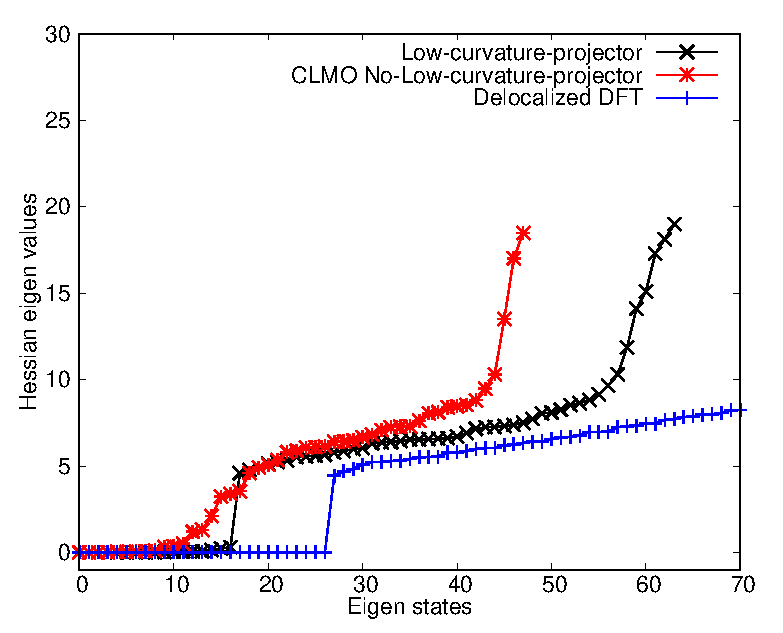
\includegraphics[width=0.4\textwidth]{Hesseig}
\caption{Eigenvalue spectra of Hessian during the optimization. The calculation is done on hexagonal CdSe lattice with 8 atoms. For the CLMO calculations the localization center is Cd$^{2+}$ ion and the domain includes one Cd$^{2+}$ and 3 Se$^{-2}$. For delocalized calculation the Hessian is for the complete system (only a portion of the eigenvalues are shown to save space). For the straight forward CLMO calculation without low-curvature-projector, the calculation won't converge and the Hessian is chosen at a stage where the energy is close to the ground state, for the other 2 cases the Hessian is chosen at convergence. PBE/DZVP level of theory is used for all cases.}
\label{sfig:hesseig}
\end{figure}

Here we give more details on our hypothesis in Eq.~(\ref{eq:residue}). First, we introduce a measure of what portion of CLMO $\ket{\psi_{yj}}$ is present outside domain $\bar{x}$:
\bea
M^{\bar{x}}_{yj} \equiv \braket{\psi_{yj}}{\psi_{yj}} - \bra{\psi_{yj}}\op{I}_{\bar{x}}\ket{\psi_{yj}}
\eea
%
Second, when constructing $\op{R}_{\bar{x}}$ in Eq.~(\ref{eq:C}), we select only those $\ket{\psi_{yi}}$ states that are significantly present on $\bar{x}$: 
\bea
M^{\bar{x}}_{yj} < t
\eea
%
where $t$ is a cutoff threshold between zero and one. 
For larger $t$, more delocalized occupied states are chosen thus reducing the dimension of the unoccupied space on $\bar{x}$ bringing $\Delta$ in Eq~\ref{eq:residue} down (Fig~\ref{sfig:t_delta}). 
The assumption is good for most weakly interacting materials but for Si where electrons are less localized the assumption is less accurate. It is important to emphasize that our method remains robust even if residues are large.

\begin{figure}
\centering
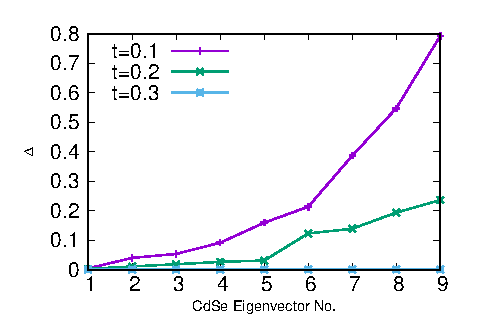
\includegraphics[width=0.3\textwidth]{t_cdse_residue}
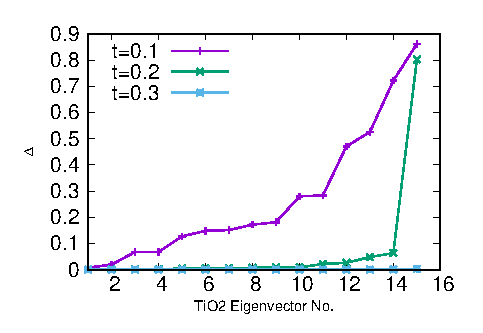
\includegraphics[width=0.3\textwidth]{t_tio2_residue}
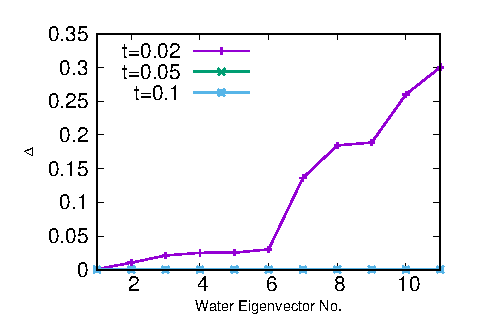
\includegraphics[width=0.3\textwidth]{t_water_residue}
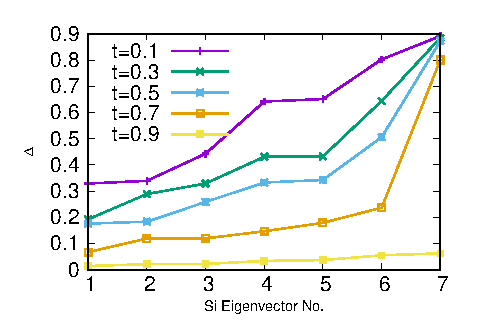
\includegraphics[width=0.3\textwidth]{t_si_residue}
\caption{$\Delta_{\bar{x}p}$ as a function of $t$, for materials studied in Fig~\ref{fig:projection}. As $t$ increases, $\Delta_{\bar{x}p}$ quickly reduces. Our assumption works well for most system except for Si.}
\label{sfig:t_delta}
\end{figure}
\end{document}
